\documentclass[a4paper,11pt]{article}

\usepackage[utf8]{inputenc}
\usepackage[cyr]{aeguill}
\usepackage[margin=0.8in]{geometry}
\usepackage{xspace}
\usepackage{amsmath}
\usepackage[english,francais]{babel}
\usepackage{url}
\usepackage{algorithm}
\usepackage{algpseudocode}
\usepackage{xcolor}
\usepackage{listings} % pour le code
\usepackage{graphicx} % pour les figures
\usepackage{subcaption}
\usepackage{csquotes}

% Redefinition de la commande \url pour pour l'utiliser dans un document en français
% sans avoir de problème avec les deux-points
% (voir http://perso.mines-albi.fr/~gaborit/latex/latex-in-french.html)
\let\urlorig\url
\renewcommand{\url}[1]{%
  \begin{otherlanguage}{english}\urlorig{#1}\end{otherlanguage}%
}
\renewcommand{\contentsname}{Sommaire} % si tableofcontents au d?but
\newcommand{\Numero}{\No}
\newcommand{\numero}{\no}

\begin{document}

\title{Compte-rendu de TP \\``Algorithme Génétique''}
\author{Jérôme FOURMOND \& Stanislas LEROY
\\ M2 Informatique – Parcours Intelligence Artificielle
\\Université Claude-Bernard Lyon 1}
\date{\today}
\maketitle

\tableofcontents
\newpage

\section{Objectif}

L'objectif de ce TP est de programmer un algorithme génétique permettant de faire évoluer une population d'individus, où chaque individu code les paramètres d'un oeil d'après la modélisation suivante (Figure \ref{fig:modelisation}) :

\begin{figure}[htbp]
\begin{center}
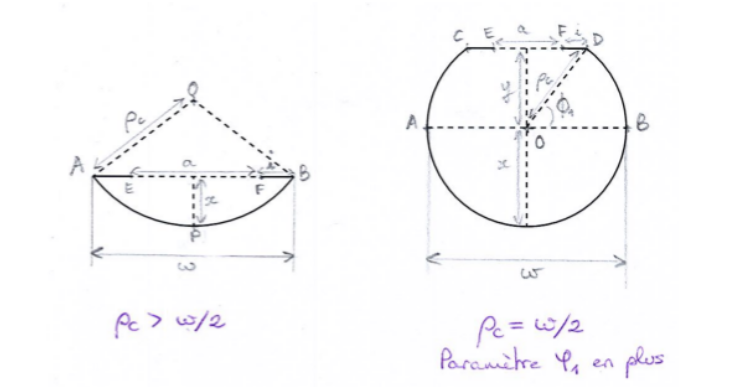
\includegraphics[width=15cm]{modelisation.png}
\caption{Modelisation}
\label{fig:modelisation}
\end{center}
\end{figure}

En outre, l'oeil peut comporter une lentille sphérique de rayon a=2 centrée sur le centre de l'ouverture (milieu du segment [EF]). Au sein de cette lentille, l'indice de réfraction $n$ suit un gradient allant de $1.35$ (à l'extérieur) à une certaine valeur $n_{0}$.

\section{Constantes}

\begin{itemize}
\item Tout au long de l'évolution, la largeur maximale de l'oeil (distance AB) reste égale à $w = 1.5$ cm,
\item L'intensité lumineuse $I$ sera prise égale à $e^{6}$.
\end{itemize}

\section{Paramètres à faire évoluer}

\begin{itemize}
\item Rayon de courbure $\rho_{c}$ : peut varier dans la plage $[w/2, 10000]$
\item Taille de l'iris $i$ : peut varier dans la plage $[0, w/2[$
\item Angle $\Phi_{1}$ : peut varier dans la plage $[0, \pi/2[$
\item Indice de réfraction $n_{0}$ au centre de la lentille : peut varier dans la plage $[1.35, 1.55]$
\end{itemize}

\section{Valeurs initiales}

\begin{itemize}
\item Rayon de courbure initial $\rho_{c} = 10000$
\item Taille initiale de l'iris $i = 0$
\item Angle $\Phi_{1}$ initial : $\Phi_{1} = 0$
\item Indice initial de réfraction au centre de la lentille $n_{0} = 1.35$
\end{itemize}

\section{Algorithme}

L'algorithme s'exécute jusqu'à ce que le nombre de générations limite soit atteint.

\subsection{Paramètres}

\begin{itemize}
\item Taille de la population : $40$
\item Nombre de générations : $50 000$
\item Taux de cross-over : $0.5$
\item Taux de mutation : $0.2$
\end{itemize}

\subsection{Processus de sélection}

\begin{enumerate}
\item Tri de la population en fonction de leur valeur de fitness
\item Récupération des probabilités de reproduction
\item Création du "camembert" en fonction de la probabilité de reproduction
\item Choix aléatoire de deux parents en fonction du camembert 
\end{enumerate}

\subsection{Processus de reproduction}

L'enfant détiendra les caractéristiques aléatoires en fonction des caractéristiques des parents et du taux de cross-over.

\subsection{Processus de mutation}

Les enfants produits muteront en fonction du taux de mutation. Une seule caractéristique de l'enfant sera modifiée (addition) par un double gaussien aléatoire.

\subsection{Processus de remplacement}

Les étapes de sélection, de reproduction et de remplacement sont effectuées jusqu'à ce que la population soit entièrement renouvelée.

\section{Programme}

Le répertoire git-hub du projet est disponible à l'adresse suivante :
\\
\url{https://github.com/jfourmond/EyeEvolution}

\subsection{Exécution}

Le programme nécessite le répertoire $resources$ contenant le fichier $indice\_refraction.dat$ pour fonctionner.
Quatre arguments sont à spécifier au programme :

\begin{itemize}
\item la taille de la population
\item le nombre de générations
\item le taux de cross-over (en pourcentage)
\item le taux de mutation (en pourcentage)
\end{itemize}

Un cinquième argument, optionnel, peut être spécifié : la graine du générateur aléatoire ($seed$).

\begin{lstlisting}
	java -jar EyeEvolution.jar [population-size] [generations] [crossover-rate] [mutation-rate] ([seed])
\end{lstlisting}

Dans le cas présent, avec les paramètres choisis, l'appel au programme via l'archive Java se fait de la façon suivante : 

\begin{lstlisting}
	java -jar EyeEvolution.jar 40 50000 50 20
\end{lstlisting}
	
\subsection{Fichier CSV}

A l'exécution, le programme produit un fichier au format $csv$ dans le répertoire $resources$ contenant les détails suivants pour chaque génération :
\begin{itemize}
\item numéro de la generation
\item taille de la population
\item taux de cross-over
\item taux de mutation
\item graine du générateur aléatoire
\item rayon de courbure moyen
\item taille de l'iris moyen
\item angle moyen
\item indice de réfraction moyen
\item fitness moyen
\item rayon de courbure du meilleur oeil
\item taille de l'iris du meilleur oeil
\item angle du meilleur oeil
\item indice de réfraction du meilleur oeil
\item fitness du meilleur oeil
\end{itemize}

\section{Résultat}

\subsection{Les différents tests}

\begin{figure}
\centering
\begin{subfigure}{.5\textwidth}
  \centering
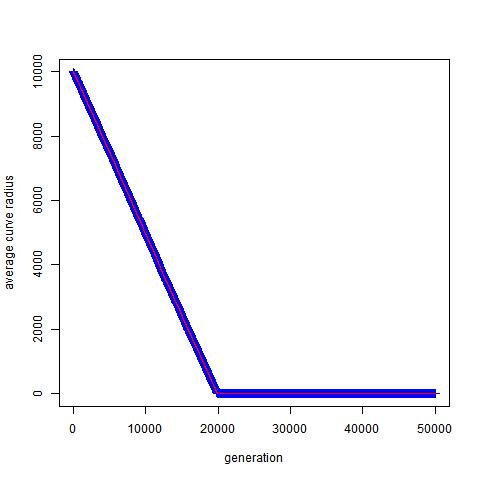
\includegraphics[width=1\linewidth]{1487422477451_evolution_average_curve_radius.jpeg}
\caption{Test 1 – Évolution du rayon de courbure moyen}
\label{fig:sub11}
\end{subfigure}%
\begin{subfigure}{.5\textwidth}
  \centering
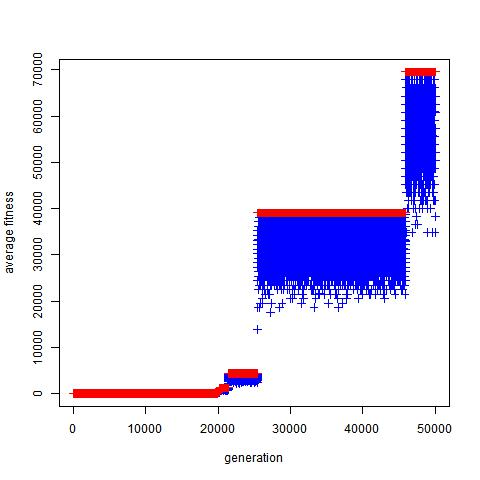
\includegraphics[width=1\linewidth]{1487422477451_evolution_average_fitness.jpeg}
\caption{Test 1 – Évolution de la fonction fitness moyenne}
\label{fig:sub12}
\end{subfigure}
\caption{}
\label{fig:test}
\end{figure}

%\begin{figure}[htbp]
%\begin{center}
%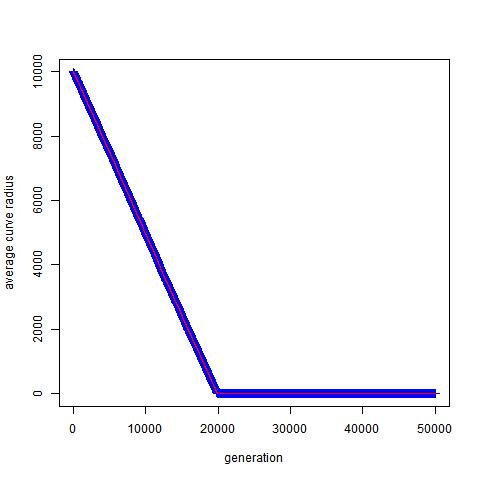
\includegraphics[width=12cm]{1487422477451_evolution_average_curve_radius.jpeg}
%\caption{a}
%\label{fig:modelisation}
%\end{center}
%\end{figure}
%
%\begin{figure}[htbp]
%\begin{center}
%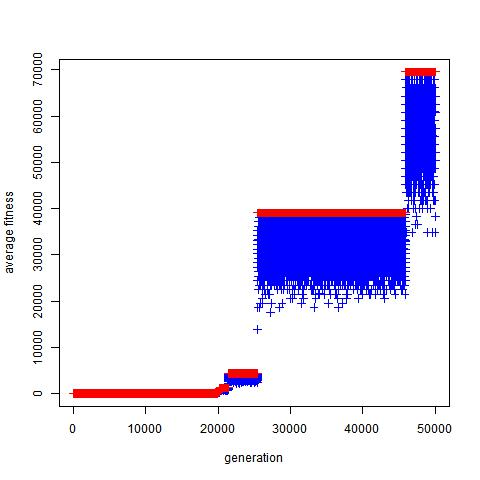
\includegraphics[width=12cm]{1487422477451_evolution_average_fitness.jpeg}
%\caption{b}
%\label{fig:modelisation}
%\end{center}
%\end{figure}



\begin{figure}
\centering
\begin{subfigure}{.5\textwidth}
  \centering
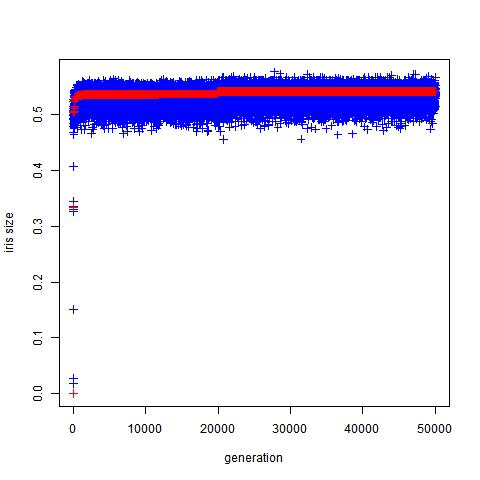
\includegraphics[width=1\linewidth]{1487422477451_evolution_average_iris_size.jpeg}
\caption{Test 1 – Évolution de la taille moyenne de l'iris}
\label{fig:sub13}
\end{subfigure}%
\begin{subfigure}{.5\textwidth}
  \centering
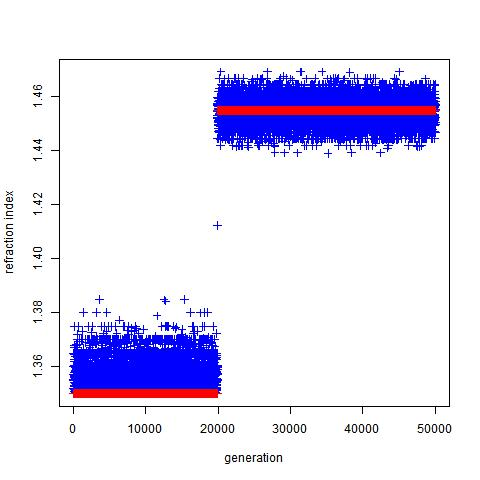
\includegraphics[width=1\linewidth]{1487422477451_evolution_average_refraction_index.jpeg}
\caption{Test 1 – Évolution de l'indice de réfraction moyen}
\label{fig:sub14}
\end{subfigure}
\caption{}
\label{fig:test}
\end{figure}

%\begin{figure}
%\begin{center}
%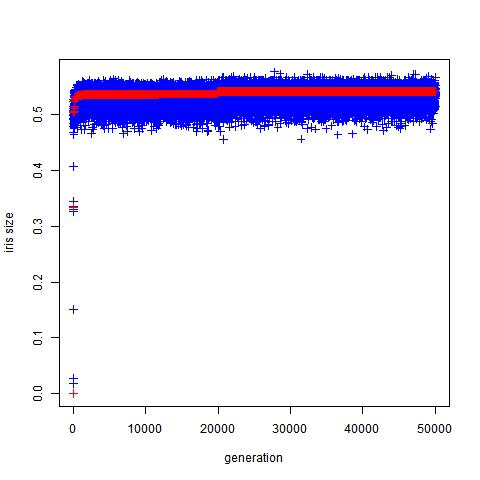
\includegraphics[width=12cm]{1487422477451_evolution_average_iris_size.jpeg}
%\caption{c}
%\label{fig:modelisation}
%\end{center}
%\end{figure}
%
%\begin{figure}[htbp]
%\begin{center}
%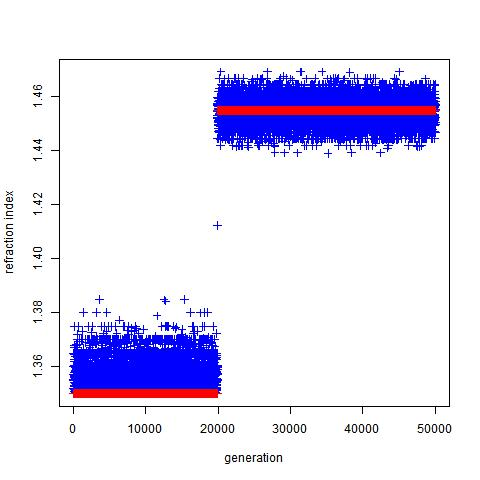
\includegraphics[width=12cm]{1487422477451_evolution_average_refraction_index.jpeg}
%\caption{d}
%\label{fig:modelisation}
%\end{center}
%\end{figure}


%\subsection{Test 2}

\begin{figure}
\centering
\begin{subfigure}{.5\textwidth}
  \centering
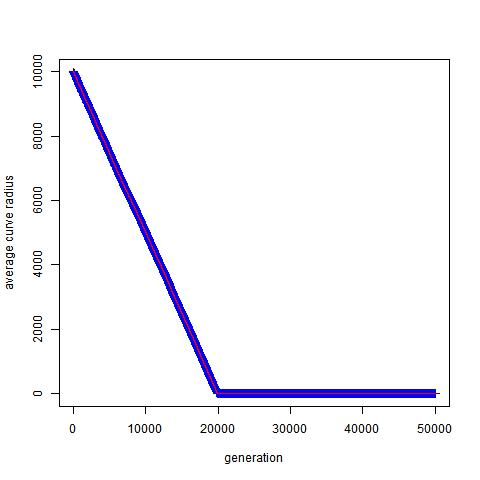
\includegraphics[width=1\linewidth]{1487424485848_evolution_average_curve_radius.jpeg}
\caption{Test 2 – Évolution du rayon de courbure moyen}
\label{fig:sub21}
\end{subfigure}%
\begin{subfigure}{.5\textwidth}
  \centering
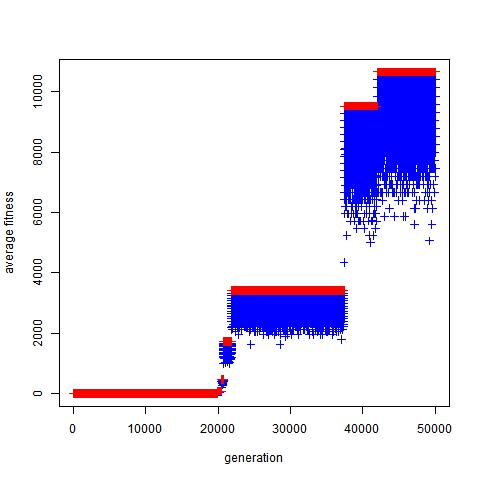
\includegraphics[width=1\linewidth]{1487424485848_evolution_average_fitness.jpeg}
\caption{Test 2 – Évolution de la fonction fitness moyenne}
\label{fig:sub22}
\end{subfigure}
\caption{}
\label{fig:test}
\end{figure}

%\begin{figure}[htbp]
%\begin{center}
%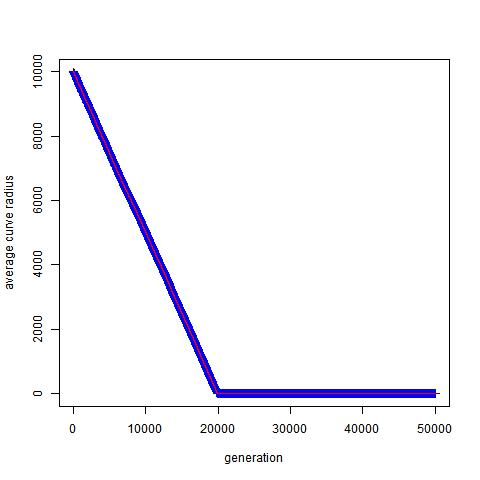
\includegraphics[width=12cm]{1487424485848_evolution_average_curve_radius.jpeg}
%\caption{a}
%\label{fig:modelisation}
%\end{center}
%\end{figure}
%
%\begin{figure}[htbp]
%\begin{center}
%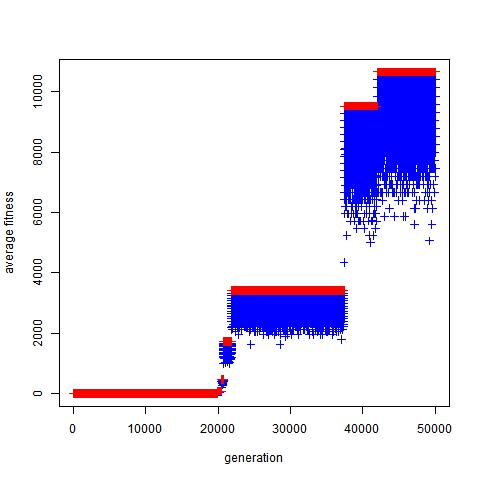
\includegraphics[width=12cm]{1487424485848_evolution_average_fitness.jpeg}
%\caption{b}
%\label{fig:modelisation}
%\end{center}
%\end{figure}



\begin{figure}
\centering
\begin{subfigure}{.5\textwidth}
  \centering
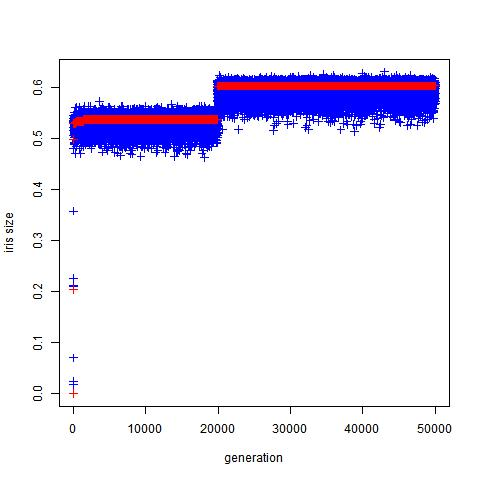
\includegraphics[width=1\linewidth]{1487424485848_evolution_average_iris_size.jpeg}
\caption{Test 2 – Évolution de la taille moyenne de l'iris}
\label{fig:sub23}
\end{subfigure}%
\begin{subfigure}{.5\textwidth}
  \centering
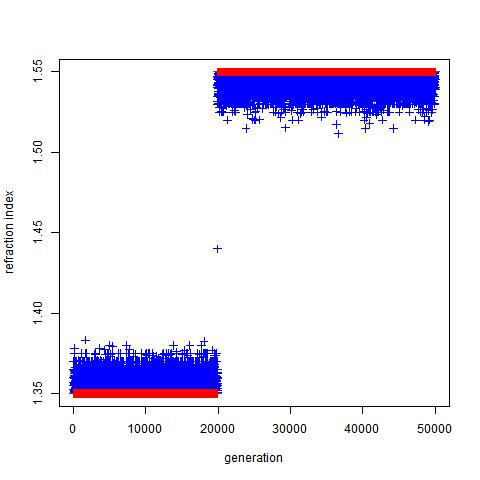
\includegraphics[width=1\linewidth]{1487424485848_evolution_average_refraction_index.jpeg}
\caption{Test 2 – Évolution de l'indice de réfraction moyen}
\label{fig:sub24}
\end{subfigure}
\caption{}
\label{fig:test}
\end{figure}

%\begin{figure}[htbp]
%\begin{center}
%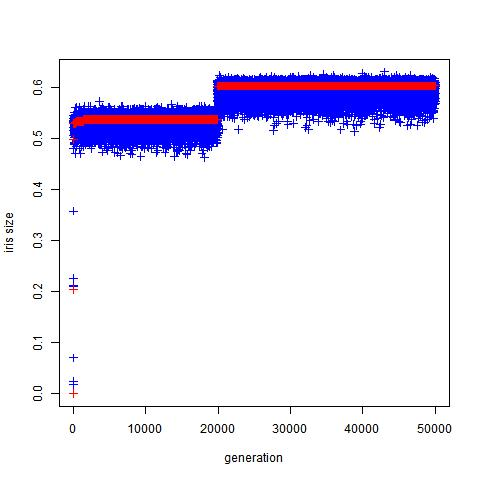
\includegraphics[width=12cm]{1487424485848_evolution_average_iris_size.jpeg}
%\caption{c}
%\label{fig:modelisation}
%\end{center}
%\end{figure}
%
%\begin{figure}[htbp]
%\begin{center}
%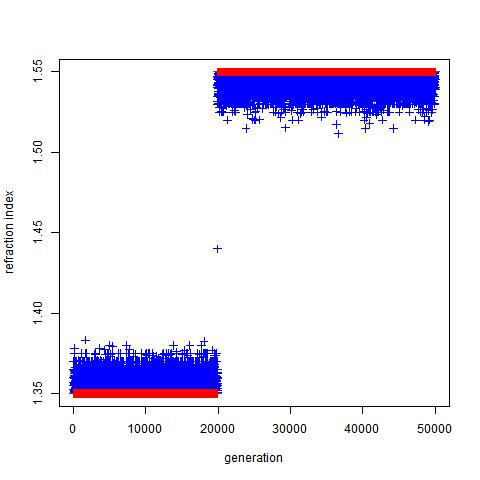
\includegraphics[width=12cm]{1487424485848_evolution_average_refraction_index.jpeg}
%\caption{d}
%\label{fig:modelisation}
%\end{center}
%\end{figure}


%\subsection{Test 3}

\begin{figure}
\centering
\begin{subfigure}{.5\textwidth}
  \centering
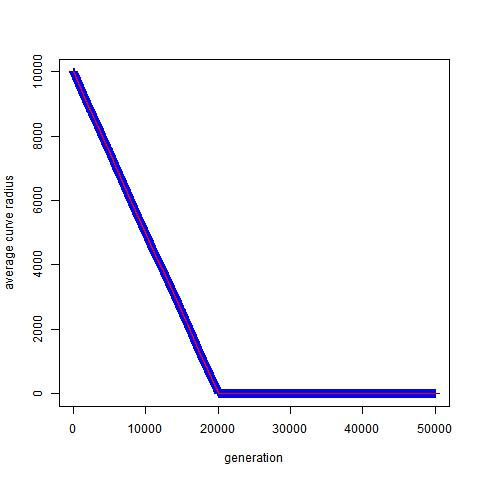
\includegraphics[width=1\linewidth]{1487424573992_evolution_average_curve_radius.jpeg}
\caption{Test 3 – Évolution du rayon de courbure moyen}
\label{fig:sub31}
\end{subfigure}%
\begin{subfigure}{.5\textwidth}
  \centering
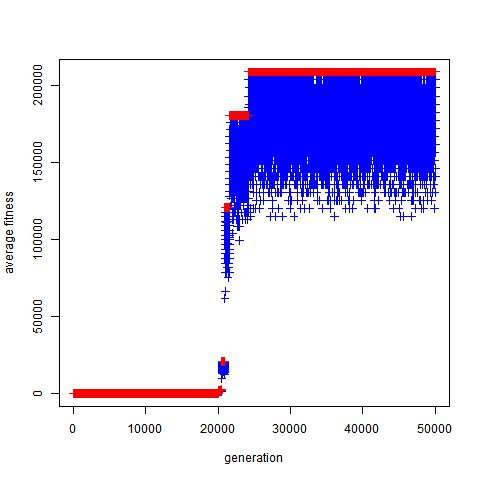
\includegraphics[width=1\linewidth]{1487424573992_evolution_average_fitness.jpeg}
\caption{Test 3 – Évolution de la fonction fitness moyenne}
\label{fig:sub32}
\end{subfigure}
\caption{}
\label{fig:test}
\end{figure}

%\begin{figure}[htbp]
%\begin{center}
%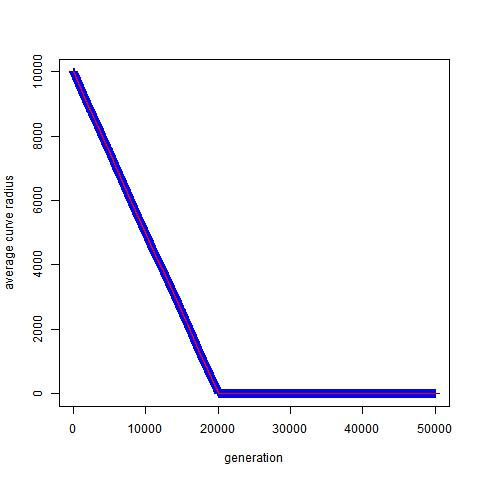
\includegraphics[width=12cm]{1487424573992_evolution_average_curve_radius.jpeg}
%\caption{a}
%\label{fig:modelisation}
%\end{center}
%\end{figure}
%
%\begin{figure}[htbp]
%\begin{center}
%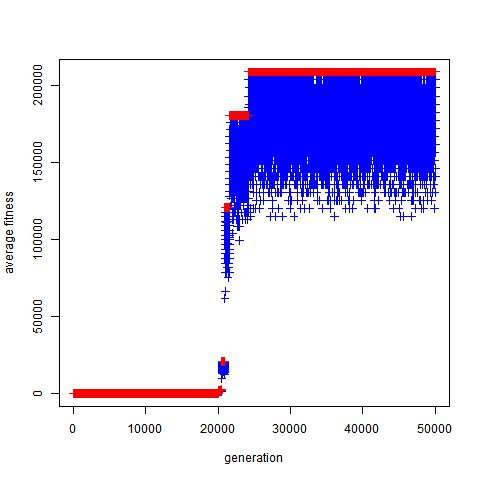
\includegraphics[width=12cm]{1487424573992_evolution_average_fitness.jpeg}
%\caption{b}
%\label{fig:modelisation}
%\end{center}
%\end{figure}


\begin{figure}
\centering
\begin{subfigure}{.5\textwidth}
  \centering
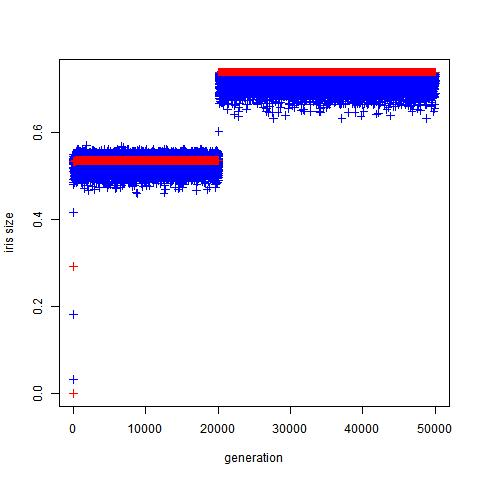
\includegraphics[width=1\linewidth]{1487424573992_evolution_average_iris_size.jpeg}
\caption{Test 3 – Évolution de la taille moyenne de l'iris}
\label{fig:sub33}
\end{subfigure}%
\begin{subfigure}{.5\textwidth}
  \centering
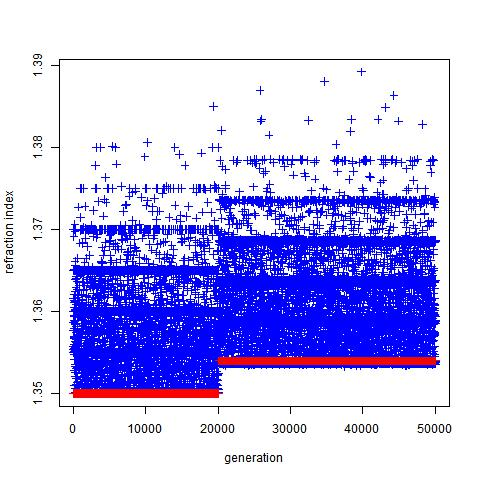
\includegraphics[width=1\linewidth]{1487424573992_evolution_average_refraction_index.jpeg}
\caption{Test 3 – Évolution de l'indice de réfraction moyen}
\label{fig:sub34}
\end{subfigure}
\caption{}
\label{fig:test}
\end{figure}

%\begin{figure}[htbp]
%\begin{center}
%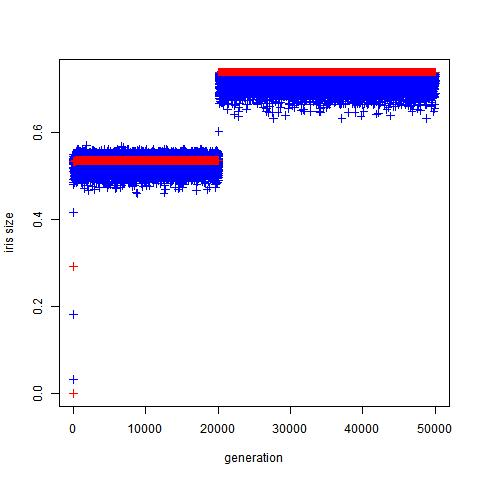
\includegraphics[width=12cm]{1487424573992_evolution_average_iris_size.jpeg}
%\caption{Évolution de la taille moyenne de l'iris}
%\label{fig:modelisation}
%\end{center}
%\end{figure}
%
%\begin{figure}[htbp]
%\begin{center}
%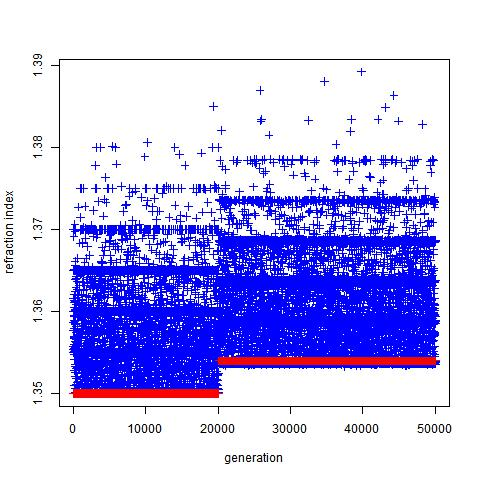
\includegraphics[width=.5\linewidth]{1487424573992_evolution_average_refraction_index.jpeg}
%\caption{Évolution de l'indice de réfraction moyen}
%\label{fig:modelisation}
%\end{center}
%\end{figure}

Les graphes concernant l'évolution des rayons de courbure moyens sont semblables entre les trois tests. Le rayon de courbure minimum est atteint au bout de 20 000 générations (voir Figures \ref{fig:sub11}, \ref{fig:sub21} et \ref{fig:sub31}).\\

Concernant la valeur moyenne de la fonction fitness, on observe que les résultats des tests 1 et 2 sont similaires et marquent une différence avec le test 3. En effet, pour deux les premiers tests (voir Figures \ref{fig:sub12} et \ref{fig:sub22}), les courbes sont des courbes en escalier. Respectivement quatre et cinq seuils sont visibles et les seuils intermédiaires sont les plus marqués. En revanche, pour le troisième test (voir Figure \ref{fig:sub32}), cinq seuils sont également présents mais les deux plus importants sont le premier (valeur minimale de la fitness moyenne) et le dernier (valeur maximale de la fitness moyenne).\\

Il existe également une distinction entre les différents tests pour la taille moyenne de l'iris. Le test 1 (voir Figure \ref{fig:sub13}) montre une évolution quasi-linéaire de cette valeur. En revanche, on observe (voir Figures \ref{fig:sub23} et \ref{fig:sub33}) une évolution avec deux paliers fortement distingués pour les tests 2 et 3.\\

Enfin, une autre distinction peut être faite concernant l'indice de réfraction moyen. À l'instar de la valeur de la fitness moyenne, les résultats des tests 1 et 2 sont similaires (voir Figures \ref{fig:sub14} et \ref{fig:sub24}) avec un net écart entre les deux paliers initiaux et finaux. À l'inverse, l'écart entre les paliers obtenus dans le test 3 (voir Figure \ref{fig:sub34}) est beaucoup moins marqué.

\subsection{Meilleurs paramètres}

\begin{figure}
\centering
\begin{subfigure}{.5\textwidth}
  \centering
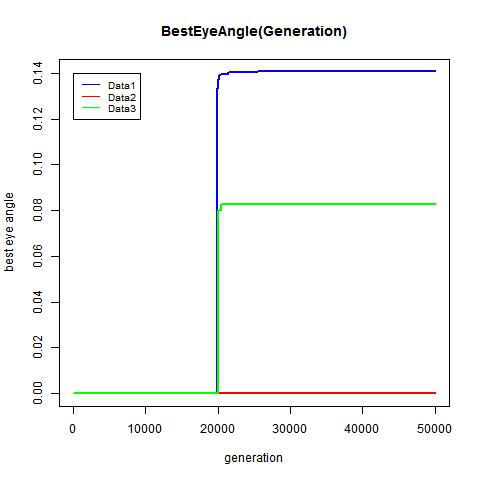
\includegraphics[width=1\linewidth]{best_eye_angle.jpeg}
\caption{Evolution de l'angle du meilleur oeil \\en fonction de la génération}
\label{fig:best_1}
\end{subfigure}%
\begin{subfigure}{.5\textwidth}
  \centering
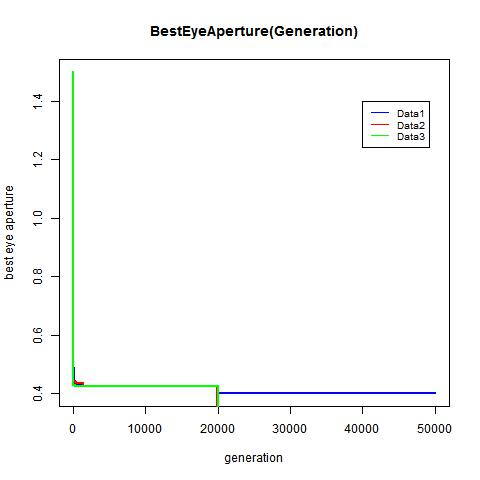
\includegraphics[width=1\linewidth]{best_eye_aperture.jpeg}
\caption{Evolution de l'ouverture du meilleur oeil \\en fonction de la génération}
\label{fig:best_2}
\end{subfigure}
\caption{}
\label{fig:test}
\end{figure}

%\begin{figure}[htbp]
%\begin{center}
%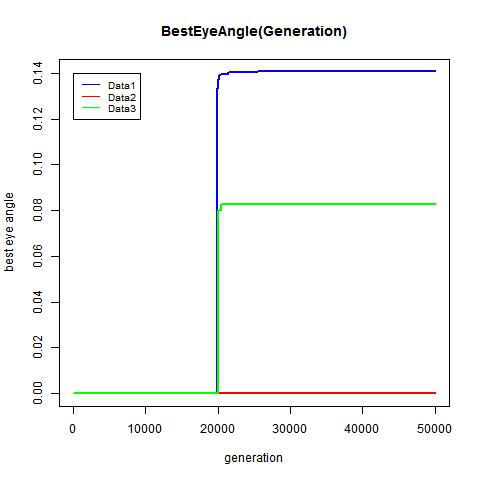
\includegraphics[width=12cm]{best_eye_angle.jpeg}
%\caption{Evolution de l'angle du meilleur oeil en fonction de la génération}
%\label{fig:modelisation}
%\end{center}
%\end{figure}

%\begin{figure}[htbp]
%\begin{center}
%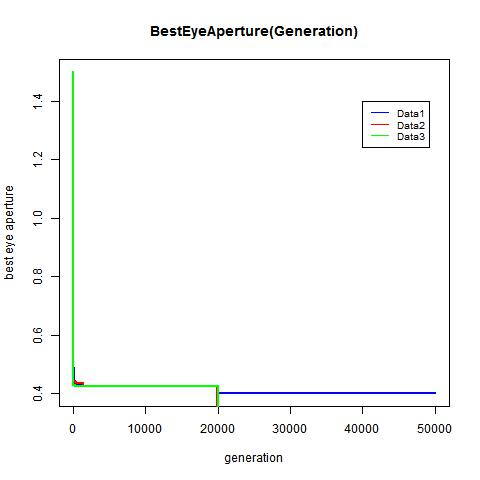
\includegraphics[width=12cm]{best_eye_aperture.jpeg}
%\caption{Evolution de l'ouverture du meilleur oeil en fonction de la génération}
%\label{fig:modelisation}
%\end{center}
%\end{figure}

\begin{figure}
\centering
\begin{subfigure}{.5\textwidth}
  \centering
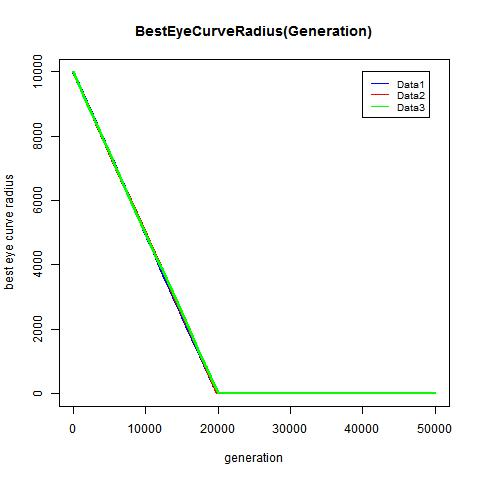
\includegraphics[width=1\linewidth]{best_eye_curve_radius.jpeg}
\caption{Evolution du rayon de courbure du meilleur oeil \\en fonction de la génération}
\label{fig:best_3}
\end{subfigure}%
\begin{subfigure}{.5\textwidth}
  \centering
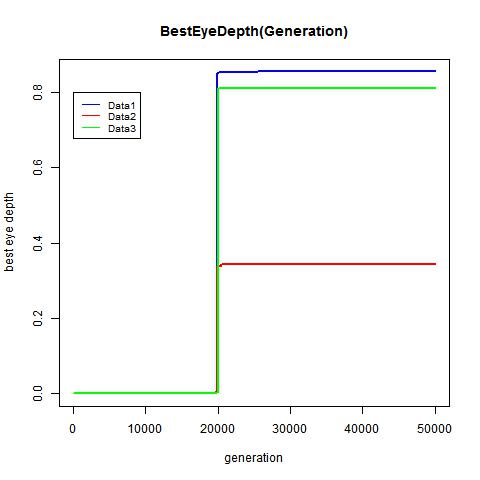
\includegraphics[width=1\linewidth]{best_eye_depth.jpeg}
\caption{Evolution de la profondeur du meilleur oeil \\en fonction de la génération}
\label{fig:best_4}
\end{subfigure}
\caption{}
\label{fig:test}
\end{figure}

%\begin{figure}[htbp]
%\begin{center}
%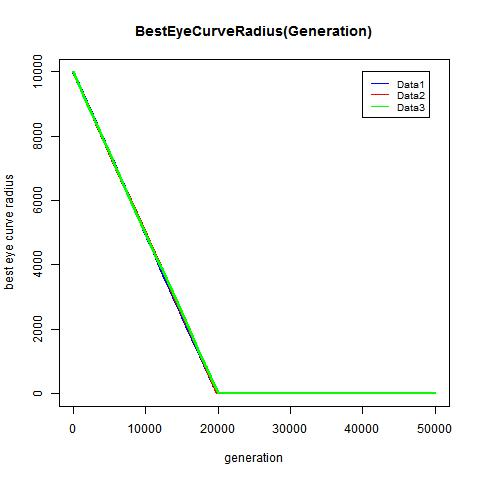
\includegraphics[width=12cm]{best_eye_curve_radius.jpeg}
%\caption{Evolution du rayon de courbure du meilleur oeil en fonction de la génération}
%\label{fig:modelisation}
%\end{center}
%\end{figure}
%
%\begin{figure}[htbp]
%\begin{center}
%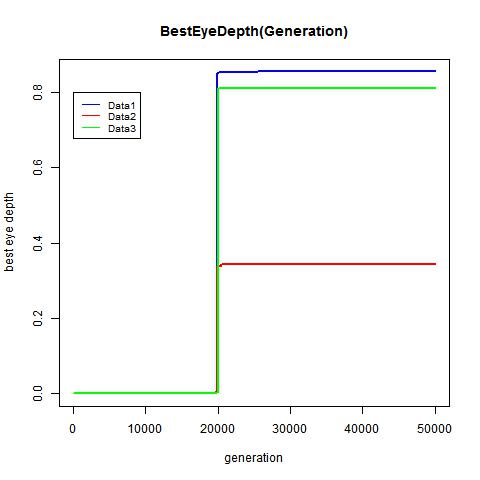
\includegraphics[width=12cm]{best_eye_depth.jpeg}
%\caption{Evolution de la profondeur du meilleur oeil en fonction de la génération}
%\label{fig:modelisation}
%\end{center}
%\end{figure}

\begin{figure}
\centering
\begin{subfigure}{.5\textwidth}
  \centering
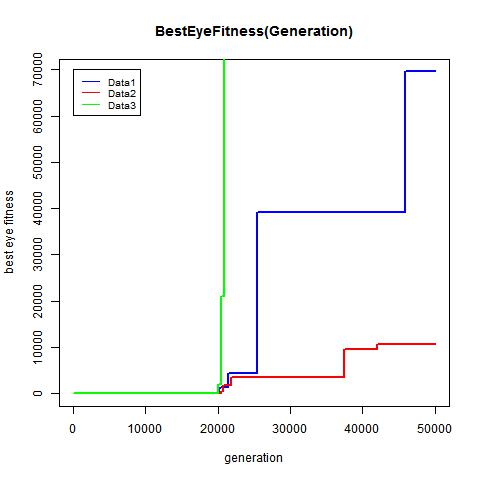
\includegraphics[width=1\linewidth]{best_eye_fitness.jpeg}
\caption{Evolution de la fitness du meilleur oeil \\en fonction de la génération}
\label{fig:best_5}
\end{subfigure}%
\begin{subfigure}{.5\textwidth}
  \centering
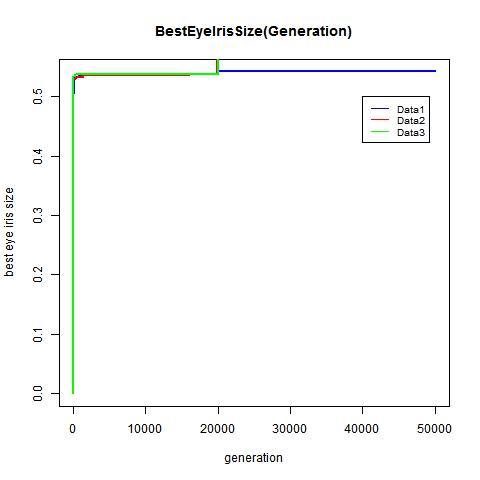
\includegraphics[width=1\linewidth]{best_eye_iris_size.jpeg}
\caption{Evolution de la taille de l'iris du meilleur oeil \\en fonction de la génération}
\label{fig:best_6}
\end{subfigure}
\caption{}
\label{fig:test}
\end{figure}

%\begin{figure}[htbp]
%\begin{center}
%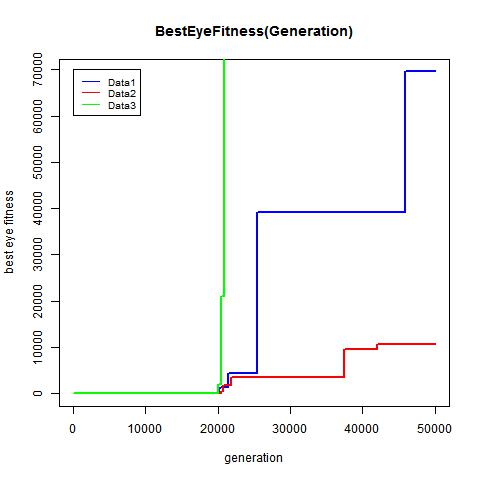
\includegraphics[width=12cm]{best_eye_fitness.jpeg}
%\caption{Evolution de la fitness du meilleur oeil en fonction de la génération}
%\label{fig:modelisation}
%\end{center}
%\end{figure}
%
%\begin{figure}[htbp]
%\begin{center}
%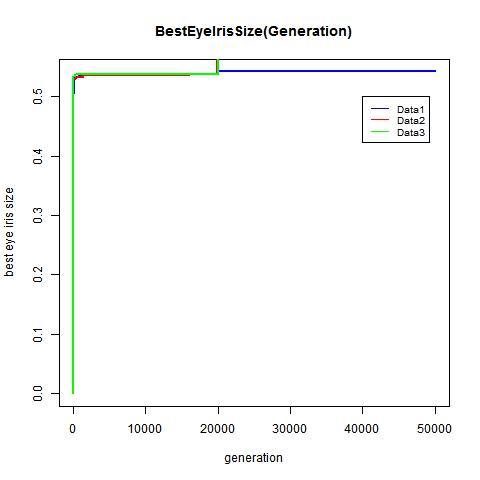
\includegraphics[width=12cm]{best_eye_iris_size.jpeg}
%\caption{Evolution de la taille de l'iris du meilleur oeil en fonction de la génération}
%\label{fig:modelisation}
%\end{center}
%\end{figure}

\begin{figure}
\centering
\begin{subfigure}{.5\textwidth}
  \centering
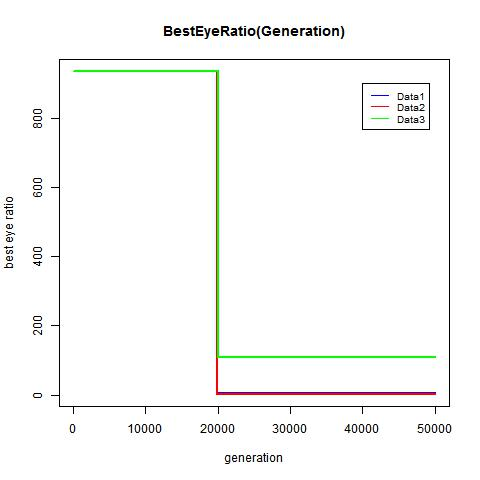
\includegraphics[width=1\linewidth]{best_eye_ratio.jpeg}
\caption{Evolution du ratio du meilleur oeil \\en fonction de la génération}
\label{fig:best_7}
\end{subfigure}%
\begin{subfigure}{.5\textwidth}
  \centering
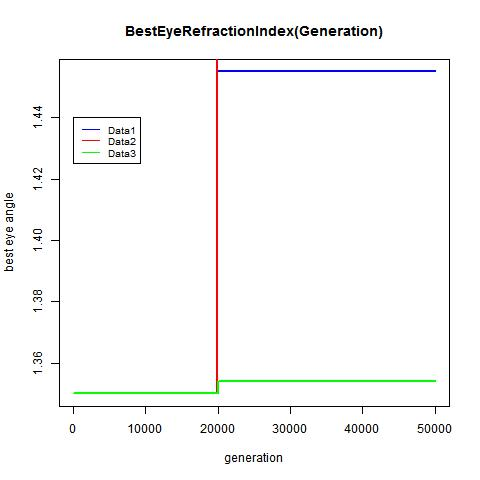
\includegraphics[width=1\linewidth]{best_eye_refraction_index.jpeg}
\caption{Evolution de l'indice de réfraction du meilleur oeil \\en fonction de la génération}
\label{fig:best_8}
\end{subfigure}
\caption{}
\label{fig:test}
\end{figure}

%\begin{figure}[htbp]
%\begin{center}
%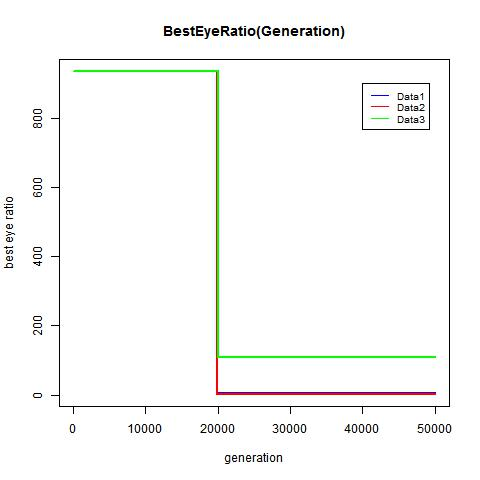
\includegraphics[width=12cm]{best_eye_ratio.jpeg}
%\caption{Evolution du ratio du meilleur oeil en fonction de la génération}
%\label{fig:modelisation}
%\end{center}
%\end{figure}
%
%\begin{figure}[htbp]
%\begin{center}
%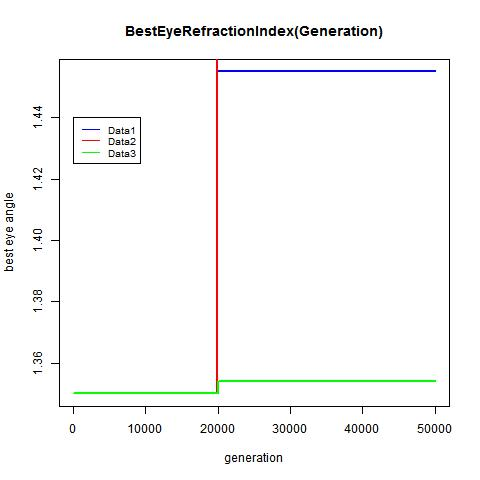
\includegraphics[width=12cm]{best_eye_refraction_index.jpeg}
%\caption{Evolution de l'indice de réfraction du meilleur oeil en fonction de la génération}
%\label{fig:modelisation}
%\end{center}
%\end{figure}

\begin{figure}[htbp]
\begin{center}
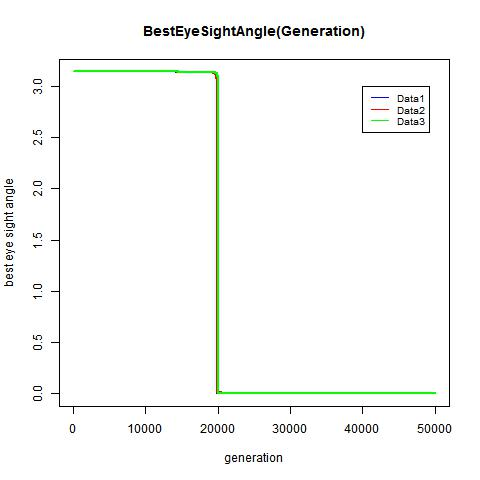
\includegraphics[width=.5\linewidth]{best_eye_sight_angle.jpeg}
\caption{Evolution de l'angle de vue du meilleur oeil en fonction de la génération}
\label{fig:best_9}
\end{center}
\end{figure}

Dans l'article de Nilson et Pelger de 1994, il est écrit : 

\begin{displayquote}
As the aperture constricts, the optical image becomes increasingly well resolved (\textit{cf}. p3).
\end{displayquote}

Les figures \ref{fig:best_2} et \ref{fig:best_4} obtenues pour les meilleurs individus illustrent ce phénomène. En effet, on observe que lorsque l'ouverture diminue (depuis la valeur 1.5 vers 0.4), la profondeur de champ augmente (de 0 vers 0.8). Les pentes des 2 courbes sont élevées, ce qui caractérise une évolution très rapide de ces paramètres. Par conséquent, les trajectoires obtenues sont effectivement similaires à celle imaginée dans l'article.

\end{document}

